\documentclass[a4paper, twoside, symmetric]{tufte-book}
\raggedbottom

%----------%
% SETTINGS %
%----------%

\makeatletter
\def\input@path{{./settings/}}
\makeatother
% settings files
\usepackage{lipsum}
\usepackage{hyperref}
\usepackage{import}  % for relative paths importing

% Packages
\usepackage{amsmath, mathtools, bm, commath}
\usepackage{physics}
\usepackage{siunitx}
\usepackage{nicematrix}

% General settings
\allowdisplaybreaks     % Allows for equations to break between pages

% Cancel-lines related
\usepackage[thicklines]{cancel}
\renewcommand\CancelColor{\color{xred}}
\newcommand{\cancelcol}[2][xred]{ % This is such a silly solution...
	\renewcommand\CancelColor{\color{#1}}
	\cancel{#2}
	\renewcommand\CancelColor{\color{xred}}
}

% Easier space-notation
\newcommand{\Rs}[1][]{\mathbb{R}^{#1}}
\newcommand{\Cs}[1][]{\mathbb{C}^{#1}}

% Set notation for vectors (currently: bold letters)
\renewcommand{\vec}[1]{\bm{#1}}
\newcommand{\uvec}[1]{\bm{\hat{#1}}}
\newcommand{\vnorm}[1]{\left\| \vec{#1} \right\|}
\newcommand{\cvec}[1]{\bm{\overline{#1}}}
\newcommand{\mat}[1]{\bm{#1}}

% Identity matrix
\newcommand{\Id}[1]{\mathbb{I}_{#1}}

% Vector operations
\newcommand{\inner}[2]{\langle #1,#2 \rangle}

% Dual space related
\newcommand{\dualspace}[1]{#1^{*}}
\newcommand{\dualvec}[1]{\vec{#1}^{*}}
\newcommand{\dualbasis}[1]{#1^{*}}
\newcommand{\dualeb}[1]{\dualvec{e}_{#1}}
\newcommand{\dualRs}[1][]{\mathbb{R}^{#1*}}
\newcommand{\dualCs}[1][]{\mathbb{C}^{#1*}}

% Row- and column-vectors: arguments separated by ";".
% Example: $\vec{a} = \colvec{1;2;3;4}$.
\makeatletter
\newcommand\rcvector[2][\\]{\ensuremath{%
  \global\def\rc@delim{#1}%
    \negthinspace\begin{bmatrix}
      \rc@vector #2;\relax\noexpand\@eolst%
    \end{bmatrix}}}
\def\rc@vector #1;#2\@eolst{%
  \ifx\relax#2\relax
    #1
  \else
    #1\rc@delim
    \rc@vector #2\@eolst%
  \fi}
\makeatother
\newcommand{\colvec}{\rcvector}
\newcommand{\rowvec}[1]{\rcvector[,\;]{#1}}
\newcommand{\GenericRowVec}[2][n]{\rowvec{#2_{1};#2_{2};\dots;#2_{#1}}}
\newcommand{\GenericColVec}[2][n]{\colvec{#2^{1};#2^{2};\vdots;#2^{#1}}}

% Colored vectors
\newcommand{\colorVec}[2]{\color{#1}{\vec{#2}}\color{black}}
\newcommand{\vred}{\colorVec{xdarkred}{v}}
\newcommand{\vblue}{\colorVec{xdarkblue}{v}}
\newcommand{\vgreen}{\colorVec{xdarkgreen}{v}}

% Basis vectors and transformations
\newcommand{\eb}[1]{\vec{e}_{#1}}
\newcommand{\ebc}[1]{\tilde{\vec{e}}_{#1}}
\newcommand{\ebr}[1]{\color{xdarkblue}\eb{#1}\color{black}}
\newcommand{\ebcr}[1]{\color{xdarkred}\ebc{#1}\color{black}}
\newcommand{\oldB}{\color{xdarkblue}B\color{black}}
\newcommand{\newB}{\color{xdarkred}\tilde{B}\color{black}}
\newcommand{\Forw}{\bm{F}}
\newcommand{\Backw}{\bm{F^{-1}}}

% Dark equal?
\newcommand{\beq}{\color{black}{=}}

% Better imaginary unit and natural base notation (to separate from variables)
\newcommand{\iu}{\mathrm{i}\mkern1mu}
\newcommand{\eu}{\mathrm{e}}
\newcommand{\Eu}[1]{\mathrm{e}^{#1}}
\newcommand{\EX}[1]{\exp\left(#1\right)}

% General nice matrix
\newcommand{\GNMatrix}[3]{
  \begin{bNiceMatrix}
    #1_{11} & #1_{12} & \dots & #1_{1#3}\\
    #1_{21} & #1_{22} & \dots & #1_{2#3}\\
    \vdots & \vdots & \Ddots & \vdots\\
    #1_{#21} & #1_{#22} & \dots & #1_{#2#3}
  \end{bNiceMatrix}
}

% Clever references (tufte-latex clashes with \autoref)
\usepackage{cleveref}
\crefname{figure}{Figure}{Figure}

% Hyperrefs etc.
\usepackage{hyperref}
\hypersetup{
  colorlinks=true,
  linkcolor=blue,
  filecolor=magenta,      
  urlcolor=cyan,
  pdftitle={Spinors for Beginners},
  pdfauthor={Peleg Bar Sapir},
}

% Packages
\usepackage{xcolor}

%%%%%%%%%%%%%%%%%%%%%%%%
%        COLORS        %
%%%%%%%%%%%%%%%%%%%%%%%%

% Normal colors
\definecolor{xred}{HTML}{BD4242}
\definecolor{xblue}{HTML}{4268BD}
\definecolor{xgreen}{HTML}{52B256}
\definecolor{xpurple}{HTML}{7F52B2}
\definecolor{xorange}{HTML}{FD9337}
\definecolor{xdotted}{HTML}{999999}
\definecolor{xgray}{HTML}{777777}
\definecolor{xcyan}{HTML}{80F5DC}
\definecolor{xpink}{HTML}{F690EA}
\definecolor{xgrayblue}{HTML}{49B095}
\definecolor{xgraycyan}{HTML}{5AA1B9}

% Dark colors
\colorlet{xdarkred}{red!85!black}
\colorlet{xdarkblue}{xblue!85!black}
\colorlet{xdarkgreen}{xgreen!85!black}
\colorlet{xdarkpurple}{xpurple!85!black}
\colorlet{xdarkorange}{xorange!85!black}
\colorlet{xdarkcyan}{xcyan!85!black}

% Very dark colors
\colorlet{xverydarkblue}{xblue!50!black}

% Document-specific colors
\colorlet{normaltextcolor}{black}
\colorlet{figtextcolor}{xblue}

% Enumerated colors
\colorlet{xcol0}{black}
\colorlet{xcol1}{xred}
\colorlet{xcol2}{xblue}
\colorlet{xcol3}{xgreen}
\colorlet{xcol4}{xpurple}
\colorlet{xcol5}{xorange}
\colorlet{xcol6}{xcyan}
\colorlet{xcol7}{xpink!75!black}

%%%%%%%%%%%%%%%%%%%%%
%        PGF        %
%%%%%%%%%%%%%%%%%%%%%

\usepackage{pgfplots}
\usepgfplotslibrary{fillbetween}%, colormaps, colorbrewer, patchplots}
\pgfplotsset{
  compat=1.16,
  %% Styles %%
  xyplane/.style = {
    axis x line=middle,
    axis y line=middle,
    xlabel=$x$,
    ylabel=$y$,
    every axis x label/.style={at={(ticklabel* cs:1.02)}, anchor=west},
    every axis y label/.style={at={(ticklabel* cs:1.02)}, anchor=south},
    axis line style={stealth-stealth, very thick, black!65},
    label style={font=\large},
    tick label style={font=\large},
    samples=100,
    xmin=-5, xmax=5,
    ymin=-5, ymax=5,
    grid=both,
    major grid style={black!15},
    minor grid style={black!10},
    xticklabels={,},
    yticklabels={,},
  },
  xynogrid/.style = {
    xyplane,
    major grid style={opacity=0},
    minor grid style={opacity=0},
  },
  xyempty/.style = {
    xyplane,
    axis line style = {draw=none},
    tick style = {draw=none},
    xlabel = {},
    ylabel = {},
    major grid style = {draw=black!0},
  },
  hyperplane1D/.style = {thick, #1},
  %% Function plots
  function/.style = {
    ultra thick, draw=#1,
  },
  filledfunction/.style = {
    function={#1}, opacity=1, fill=#1, fill opacity=0.3,
  },
}

%%%%%%%%%%%%%%%%%%%%%%
%        TikZ        %
%%%%%%%%%%%%%%%%%%%%%%

\usepackage{tikz, tikz-3dplot}
\usetikzlibrary{calc, shapes, intersections, backgrounds}
\tikzset{
  %% Styles %%
  vector/.style = {#1, ultra thick, -stealth, cap=round},
  pics/ruler/.style n args = {5}{
      code = {
          % Parameters
          \pgfmathsetmacro{\width}{#1}
          \pgfmathsetmacro{\height}{#2}
          \pgfmathsetmacro{\yMaj}{\height/3}
          \pgfmathsetmacro{\yMid}{\yMaj*0.7}
          \pgfmathsetmacro{\yMin}{\yMaj*0.5}
          \pgfmathsetmacro{\dxMaj}{#3}
          \pgfmathsetmacro{\dxMin}{\dxMaj*0.1}
          \pgfmathsetmacro{\maxMajGrad}{ceil((\width-2)/\dxMaj)}
          \pgfmathsetmacro{\maxMidGrad}{\maxMajGrad-0.5}
          \pgfmathsetmacro{\maxMinGrad}{(\maxMajGrad-1)*10}

          % Main rectangle
          \draw[thick, fill=#4] (0,0) rectangle (\width,\height);

          % Graduations
          % Major
          \foreach \x [count=\k from 0] in {1,2,...,\maxMajGrad}
              \draw[thick] ({\x*\dxMaj}, \height) -- ++(0.0,-\yMaj) node[below] (g\k) {$\k$};
          % Middle
          \foreach \y in {1.5,2.5,...,\maxMidGrad}
              \draw[thick] ({\y*\dxMaj}, \height) -- ++(0.0,-\yMid);
          % Minor
          \foreach \z in {1,2,...,\maxMinGrad} 
              \draw[thin] ({\dxMaj+\z*\dxMin}, \height) -- ++(0.0,-\yMin);

          % units label
          \node[below of=g0, font=\small, yshift={11*\height}] {#5};
      }
  }
}
\newcommand{\rulerTwoD}[6]{
  \pgfmathsetmacro{\Vx}{#1};
  \pgfmathsetmacro{\Vy}{#2};
  \pgfmathsetmacro{\a}{#3};
  \pgfmathsetmacro{\scale}{3*\a/sqrt(\Vx*\Vx+\Vy*\Vy)};
  \foreach \b in {-#4,...,#4}
    \addplot[very thick, #5] {-(\Vx/\Vy)*x+(\b/\a)};
}

% section numbering
\setcounter{secnumdepth}{2}

% Chapter title
\titleformat{\chapter}
[block]% shape
{\relax\ifthenelse{\NOT\boolean{@tufte@symmetric}}{\begin{fullwidth}}{}}% format applied to label+text
{\itshape\huge\thechapter}% label
{1em}% horizontal separation between label and title body
{\huge\rmfamily\itshape}% before the title body
[\ifthenelse{\NOT\boolean{@tufte@symmetric}}{\end{fullwidth}}{}]% after the title body

\usepackage{enumitem}
\usepackage{fontawesome}

% Bold text itemize/enumerate
% Taken from an answer to the TeX StackExchange question #266225
\newenvironment{descitemize}
{\begin{description}[leftmargin=*, before=\let\makelabel\descitemlabel]}
{\end{description}}
\newcommand{\descitemlabel}[1]{\textbullet\ \textbf{#1}:}

\usepackage[most]{tcolorbox}

\tikzset{
	second box/.style={
		anchor=east,
		text=white,
		rounded corners,
		fill=#1,
		xshift=-4mm,
	},
}

\tcbset{
	common/.style n args={2}{
		colframe={#1},
		colback={#1!5},
		colbacktitle={#1},
		lower separated=false,
		coltitle=white,
		boxrule=1pt,
		fonttitle=\bfseries,
		enhanced,
		breakable,
		top=8pt,
		before skip=1em,
		after skip=2em,
		attach boxed title to top left={
			yshift=-0.25cm,
			xshift=0.38cm,
		},
		boxed title style={
			boxrule=0pt,
			colframe=white,
			arc=5pt,
			outer arc=4pt,
		},
		separator sign={~~},
		overlay unbroken and last={
			\node[text=white, align=right, rounded corners, fill=#1, xshift=-4mm, minimum height=6mm, anchor=east] at (frame.south east) {#2};
		}
	},
	defstyle/.style={
		common={xpurple}{$\bm{\pi}$},
	},
	theoremstyle/.style={
		common={xgraycyan}{$\multimapdotbothA$},
	},
	lemmastyle/.style={
		common={xgrayblue}{$\multimap$},
	},
	proofstyle/.style={
		common={xgreen}{\textbf{QED}},
	},
	examplestyle/.style={
		common={xblue}{\faStar},
	},
	notestyle/.style={
		common={xred}{\textbf{!}},
	},
	challengestyle/.style={
		common={xorange}{\textbf{?}},
	},
	quotestyle/.style={
		common={gray}{\textbf{"}},
	},
}

\newtcbtheorem[auto counter, number within=chapter]{definition}{Definition}{defstyle}{def}
\newtcbtheorem[auto counter, number within=chapter]{theorem}{Theorem}{theoremstyle}{theorem}
\newtcbtheorem[auto counter, number within=chapter]{lemma}{Lemma}{lemmastyle}{lemma}
\newtcbtheorem[auto counter, number within=chapter]{proof}{Proof}{proofstyle}{proof}
\newtcbtheorem[auto counter, number within=chapter]{example}{Example}{examplestyle}{example}
\newtcbtheorem[auto counter, number within=chapter]{note}{Note}{notestyle}{note}
\newtcbtheorem[auto counter, number within=chapter]{challenge}{Challenge}{challengestyle}{challenge}
\newtcbtheorem[]{nquote}{Quote}{quotestyle}{quote}

% \usepackage[backend=biber]{biblatex}
% \addbibresource{refs/references.bib}


%----------%
% DOCUMENT %
%----------%

\begin{document}
% \part{Tests}
% \chapter{General layout test}
% \section{This is a title}\label{sec:title}
\lipsum[2-2]

\begin{marginfigure}
    \begin{center}
    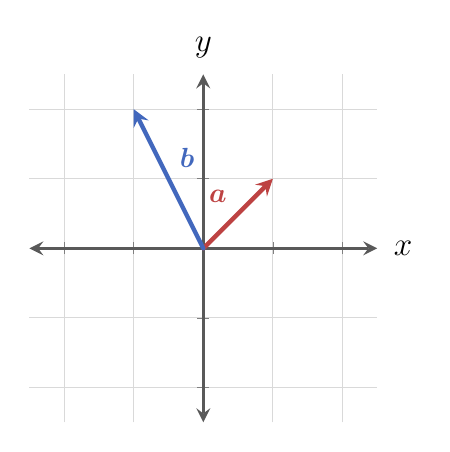
\begin{tikzpicture}
    \begin{axis}[
        xyplane,
        width=6cm, height=6cm,
    ]
        \draw[vector={xred}] (0,0) -- (2,2) node[midway, above left] {$\vec{a}$};
        \draw[vector={xblue}] (0,0) -- (-2,4) node[midway, above right] {$\vec{b}$};
    \end{axis}
    \end{tikzpicture}
    \end{center}
    \caption{A margin figure.}
    \label{fig:margin_figure}
\end{marginfigure}

This is a manualy-typed text. It even points to a figure (see \autoref{fig:margin_figure}).


\makeatletter

%% -- PART 1: Background -- %%
\part{Background Topics}

% Linear algebra
\chapter{Linear Algebra}
\def\input@path{{./parts/background/linear_algebra}}
\section{Preface}
\newthought{The goal of this chapter} is not to teach you, the reader, linear algebra from scratch - nor to be a thorough source of information on the topic. Rather, my aim is to overview the topic in such a way that new-comers, as well as those who studied linear algebra in an undergraduate university course, will gain the important insights of the topic needed for understanding the rest of the background material and spinors as well.

Instead of teaching the topic from the ground-up, like mathematicians tend to do\sidenote{In my view, courses that \enquote{build} linear algebra step-by-step give the students good knowledge of the structures of vector spaces, but tend to miss the intuitive view of what these structures can \textit{do}. This is exactly the difference between the \enquote{pure} mathematics of the mathematician and the mathematics as a tool of the scientist.}, I prefer to stick to the geometric interpretation of the vector spaces $\Rs[2]$ and $\Rs[3]$ (and to a lesser extent $\Rs[n]$ in general). These interpretations can be visualized relatively easily, and thus help in setting up the needed intuition in the student's mind, which becomes handy when the topic turns to more abstract constructs (such as for example vector spaces of matrices or functions).

In my personal experiences, when I was studying the topic I completely failed to understand it (and indeed, failed the courses I took) until it \enquote{clicked} for me in regards to 2- and 3-dimensional real spaces, i.e. - visible geometry. Then I didn't even have to study for exams anymore, as everything became clear enough to grasp and develop on the spot even during an exam (except for later, more advances concepts). That is why, for example, I absolutely adore courses and study materials of the topic\sidenote{And other mathematical topics as well.} which use animation, such as \textit{3Blue1Brown} great video essay series \href{https://www.3blue1brown.com/topics/linear-algebra}{Essence of linear algebra}\sidenote{Temporary sidenote which should become a citation for the mentioned 3B1B video series}.

There are very few proofs in this chapter, and those that are shown are not completely rigorous. For more in-depth materials, see the last section (further read). With that out of the way - let's begin!
\newpage

% \section{Vector Spaces Beyond $\Rs[n]$}
\subsection{Why go beyond $\Rs[n]$?}
\newthought{As mentiond before}, I'm a strong believer in studying linear algebra starting from the intuitive and easy to visualize geomteric cases - that is, the spaces $\Rs[2]$ and $\Rs[3]$. The generalization to $\Rs[n]$ is then pretty straight forward. However, there is nothing special about $\Rs[n]$ as a vector space (or even $\Cs[n]$ for that matter) - any set of objects with similar strucure to $\Rs[n]$ can be analyzed to yield equivalent properties.

What do I mean by a set having a \enquote{similar structure} to $\Rs[n]$? This can answered by looking at the most fundamental properties of $\Rs[n]$ and looking for other mathematical objects which have these (or equivalent) properties. In this chapter we will find out that there are, in fact, many such objects - for example matrices, polynomials, and even (some) functions. Understanding the similarities to $\Rs[n]$ will then allow us to derive their own version of the ideas linear algebra gifts us with in regard to $\Rs[n]$ - such as (but not limited to!) meaningful subspaces, change of basis, eigen values/vectors and so on.

These ideas will be proven as quite strong tools for any scientific field based in mathematics. In fact, many of the known advanced mathematical topics such as differential equations, Fourier series and transforms, graph theory and more - all use linear algebra on some mathematical structures except $\Rs[n]$.

\subsection{The Fundamental Properties of $\Rs[n]$}
So what are the fundamental properties of $\Rs[n]$ I mentioned? They are the following (note - some will seem trivial to even mention, but are important for generalization):
\begin{descitemize}
    \item[Closure of vector addition] adding together any two vectors in $\Rs[n]$ always results in a vector in $\Rs[n]$. Mathematically:
    \begin{equation}
        \forall\vec{u},\vec{w}\in\Rs[n]: \vec{v}+\vec{w}=\vec{a}\in\Rs[n].
        \label{eq:vector_addition_closure}
    \end{equation}
    (Read: \enquote{for any vectors $\vec{u}$ and $\vec{w}$ in $\Rs[n]$, their sum, here called $\vec{a$}, is also a vector in $\Rs[n]$}.)
    
    \item[Commutativity of vector addition] it doesn't matter in which order we add to vectors together, the result is always the same (remember the parallelogram rule):
    \begin{equation}
        \vec{u}+\vec{v}=\vec{v}+\vec{u}.
        \label{eq:vector_addition_commutative_2}
    \end{equation}

    \item[Associativity of vector addition] the order of adding multiple vectors also does not matter: for any three vectors $\vec{u},\ \vec{v},\ \vec{w}$ in $\Rs[n]$,
    \begin{equation}
        \vec{u}+\left(\vec{v}+\vec{w}\right) = \left(\vec{u}+\vec{v}\right)+\vec{w}.
        \label{eq:vector_addition_associative}
    \end{equation}
    
    \item[Existence of zero] there's always a vector which is neutral to addition - this is of course the zero vector $\vec{0}$:
    \begin{equation}
        \forall \vec{u}\in\Rs[n]:\ \vec{u}+\vec{0}=\vec{0}+\vec{u}=\vec{u}.
        \label{eq:vector_zero_existence}
    \end{equation}

    \item[Existence additive inverse] any vector $\vec{v}\in\Rs[n]$ has an inverse:
    \begin{equation}
        \forall \vec{v}\in\Rs[n]:\ \exists\left(-\vec{v}\right), \vec{v}+\left(-\vec{v}\right) = \vec{0}.
        \label{eq:vector_zero_addition}
    \end{equation}

\item[Closure of scalar multiplication] the result of scaling any vector $\vec{v}\in\Rs[n]$ by a real number $\lambda\in\Rs$ is also a vector in $\Rs[n]$:
    \begin{equation}
        \forall\vec{v}\in\Rs[n] \text{and}\ \forall\lambda\in\Rs:\ \lambda\vec{v}\in\Rs[n].
        \label{eq:scalar_multiplication_closure}
    \end{equation}

\item[Associativity of scalar multiplication] the order of scaling a vector $\vec{v}$ by any two scalars $\lambda,\mu$ doesn't matter - the result would be the same no matter if we first scale $\vec{v}$ by $\lambda$ and then by $\mu$, or first scale $\vec{v}$ by $\mu$ and then by $\lambda$:
    \begin{equation}
        \left(\lambda\vec{v}\right)\cdot\mu = \lambda\cdot\left(\mu\vec{v}\right).
        \label{eq:scalar_multiplication_associative}
    \end{equation}

    \item[Existnce of unity] the number $1$ is neutral with regards to vector scaling: for any vector $\vec{v}\in\Rs[n]$, scaling $\vec{v}$ by $1$ results in $\vec{v}$:
        \begin{equation}
            \forall \vec{v}\in\Rs[n]: 1\vec{v}=\vec{v}.
            \label{eq:scalar_multiplication_unity}
        \end{equation}

    \item[Distributive laws] vector addition and scaling are distributive together with addition of scalars, i.e. for any $\vec{v},\vec{u}\in\Rs[n]$ and $\lambda,\mu\in\Rs$:
        \begin{align}
            \lambda\left(\vec{v}+\vec{w}\right) &= \lambda\vec{v} + \lambda\vec{w},\ \text{and}\\ \left(\lambda+\mu\right)\vec{v} &= \lambda\vec{v} + \mu\vec{v}.
            \label{eq:label}
        \end{align}
\end{descitemize}


%% !!! CORRECT ISSUE with \cref and example environment !!! %%

% Outline:
% * Linear algebra on R^n prooved useful (e.g. linear transformations, basis sets, etc.). It would be nice to have similar results for other structures.
% * To find more structures for which we can derive similar ideas, we first need to overview the fundamental properties of vectors in R^n, and see if there are any other structures with similar properties.
% * Fundamental properties
% * Matrices have the same properties! (+elaboration)
% * Polynomial functions have the same properties! (+elaboration)
% * Functions have the same properties! (+elaboration)
% * Using these properties to define a vector space + short discussion.

\section{Change of Coordinates}
\newthought{In introductory linear algebra courses} you should have learned about change of coordinate systems: a coordinate system is just another name for a basis set of whatever vector space is used (in this section it's $\Rs[n]$). A change of coordinate system is the transformation of vectors from being represented in one basis set $B=\left\{\eb{1},\eb{2},\dots,\eb{n}\right\}$ to being represented in another basis set $\tilde{B}=\left\{\ebc{1},\ebc{2},\dots,\ebc{n}\right\}$. Since such transformations are linear they are commonly represented in a matrix form.

In this section we will discuss \textit{how} vectors and their components change under change of basis sets. There are many components involved in these kind of transformations, which causes them to be quite confusing. I will therefore color code the equations consistently as a visual guide. In addition, I will always introduce the $\Rs[2]$ case first, before giving the generalized form for $\Rs[n]$.

\subsection{Change of basis set in $\Rs[2]$}
Suppose we use the standard basis set to represent $\Rs[2]$:
\begin{equation}
    \color{xdarkblue}
    B = \left\{\eb{1},\eb{2}\right\} = \left\{\colvec{1;0},\colvec{0;1}\right\},
    \color{black}
    \label{eq:std_basis_set_R2}
\end{equation}
and we want to change our coordinate system to use the following basis set:
\begin{equation}
    \color{xdarkred}
    \tilde{B} = \left\{\ebc{1},\ebc{2}\right\} = \left\{\colvec{2;1},\colvec{-\frac{1}{2};\frac{1}{4}}\right\}.
    \color{black}
    \label{eq:transformed_basis_set_R2}
\end{equation}
(the two basis sets are shown in \cref{fig:two_basis_sets_R2})

\begin{marginfigure}[0\baselineskip]
    \begin{center} 
        \begin{tikzpicture}
            \begin{axis}[
                xynoaxes,
                width=6cm, height=6cm,
                xmin=-0.75, xmax=2.5,
                ymin=-0.75, ymax=2.5,
                xtick={0,1,2}, extra x ticks=0,
                ytick={0,1,2}, extra y ticks=0,
                major grid style={dotted, draw=black!50},
            ]
                \draw[vector={xdarkblue}] (0,0) -- (1,0) node[pos=1.2] {$\eb{1}$};
                \draw[vector={xdarkblue}] (0,0) -- (0,1) node[pos=1.2] {$\eb{2}$};
                \draw[vector={xdarkred}] (0,0) -- (2,1) node[pos=1.075] {$\ebc{1}$};
                \draw[vector={xdarkred}] (0,0) -- (-0.5,0.25) node[pos=1.3] {$\ebc{2}$};
            \end{axis}
        \end{tikzpicture}
    \end{center}
    \caption{The standard basis set $\color{xdarkblue}{B}$ and a new basis set $\color{xdarkred}{\tilde{B}}$ shown together.}
    \label{fig:two_basis_sets_R2}
\end{marginfigure}

\vspace{1.5em}
\begin{equation}
    \Forw =
    \begin{bmatrix}
        \tikzmark{ebc1}{2} & \tikzmark{ebc2}{-\frac{1}{2}} \\
        1 & \frac{1}{4}
    \end{bmatrix}.
    \label{eq:forward_trans}
\end{equation}

\tikz[overlay, remember picture]{
    \node[xdarkred] (ebc1txt) at ($(pic cs:ebc1)+(4pt,1cm)$) {$\ebc{1}$};
    \node[xdarkred] (ebc2txt) at ($(pic cs:ebc2)+(4pt,1cm)$) {$\ebc{2}$};
    \draw[-stealth, xdarkred] (ebc1txt) -- ($(pic cs:ebc1)+(4pt,10pt)$);
    \draw[-stealth, xdarkred] (ebc2txt) -- ($(pic cs:ebc2)+(4pt,10pt)$);
}

Now, if we want to transform $\ebc{1}$ and $\ebc{2}$ into $\ebcr{1}$ and $\ebcr{2}$ using $\Forw$, we simply multiply them by $\Forw$:
\begin{align}
    \ebcr{1} &= \Forw \ebr{1},\\\nonumber
    \ebcr{2} &= \Forw \ebr{2}.
    \label{eq:transforming_ebs}
\end{align}

To make \cref{eq:transforming_ebs} more concise, we can collect the two vectors into a matrix disguised as a row vecor:
\begin{equation}
    \color{xdarkblue}
    \eb{} =
    \begin{bmatrix}
        1 & 0\\
        0 & 1
    \end{bmatrix} = \rowvec{\eb{1},\eb{2}}
    \color{black}.
    \label{eq:eb_matrix}
\end{equation}

We then get that \cref{eq:transforming_ebs} can be written in vector-matrix notation as
\begin{equation}
    \color{xdarkred}\ebcr{} = \rowvec{\eb{1};\eb{2}}
    \color{black} =
    \color{xdarkblue}\rowvec{\eb{1};\eb{2}}
    \color{black}
        \begin{bmatrix}
            2 & -\frac{1}{2}\\
            1 & \frac{1}{4}
        \end{bmatrix}
        = \rowvec{2\ebr{1}+\ebr{2};-\frac{1}{2}\ebr{1}+\frac{1}{4}\ebr{2}}.
    \label{eq:full_forward_trans}
\end{equation}

The reverse transformation can be calculated by applying the inverse transformation $\Backw$ on \cref{eq:full_forward_trans}:
\begin{equation}
    \color{xdarkred}\rowvec{\ebc{1};\ebc{2}}
    \color{black}\Backw =
    \left(
        \color{xdarkblue}\rowvec{\eb{1};\eb{2}}
        \color{black} \Forw
    \right)\Backw =
    \color{xdarkblue}\rowvec{\eb{1};\eb{2}}.
    \label{eq:eb_from_ebc}
\end{equation}
(where $\Backw=\begin{bmatrix}\frac{1}{4} & \frac{1}{2}\\ -1 & 2\end{bmatrix}$)

\subsection{Contravarience behabiour of vectors}

\section{Dual Vectors and Dual Spaces}
% Overview:
% Measuring vectors: rulers. How they look like in R2, R3, etc.
% Every ruler can be represented using a specific vector in Rn (direction + density). The measurement is then done via the inner product.
% These inner products actually represent all possible linear functionals Rn->R. They make a linear space on their own.
% Define general idea of dual spaces.
% Basis sets and change of basis - covarience, contravarience and all that.
% relevant SE answers: https://math.stackexchange.com/questions/3749/why-do-we-care-about-dual-spaces, https://math.stackexchange.com/a/3751/849224
% Citation in bibliography file

\subsection{Linear measurements and rulers\\(or: why do we care about dual vectors?)}
\newthought{Frequently in linear algebra} we want to measure vectors. A measure in this context is a way to assign each vector a real number which somehow reflects its properties (i.e. direction and/or magnitude). Mathematically, we are looking for a function $\phi:\Rs[n]\to\Rs$ - we feed it a vector, and it returns some measurement.

One common way to measure vectors is using the norm: the norm of a vector in $\Rs[n]$ using the standard basis set $\eb{1},\eb{2},\dots,\eb{n}$ is given by
\begin{equation}
    \vnorm{v} = \sqrt{v_{1}^{2}+v_{2}+\dots+v_{n}^{2}},
    \label{eq:std_norm}
\end{equation}
where the numbers $v_{1},v_{2},\dots,v_{n}$ are the components in each of the respective basis vectors.

While the norm does tell us something useful about a vector, it has two drawbacks: it doesn't tell us anything about the vector's orientation in space, and even worse - it is not linear. We can try and simplify the calculation of the norm by dropping the square root and calculating the \textit{square norm}, but that too isn't linear, nor does it tell us anything about the vector's orientation.

Another way of measuring vectors is by using \textit{rulers}. Rulers are nothing more than a set of graduation lines with an orientation in space (\cref{fig:rulers}). We can therefore represent a ruler using a vector: the magnitude of the vector is the frequency of the graduation lines, while its direction is the direction of the ruler (which is orthogonal to the graduation lines). To not confuse ruler vectors with \enquote{regular} vectors, I will denote ruler vectors using a greek letter and an asterisk, e.g. $\dualvec{\alpha}$.

\begin{marginfigure}[-35\baselineskip]
    \begin{center} 
        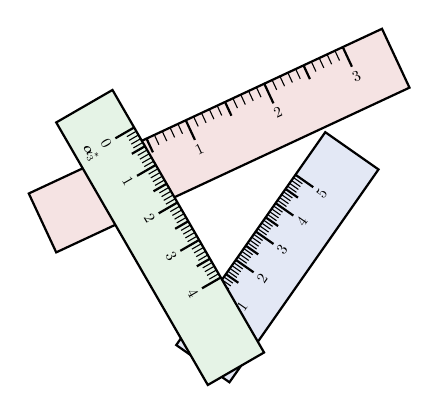
\begin{tikzpicture}[scale=0.55]
            \path pic[rotate=25, transform shape] (A) {ruler={9}{1.5}{2}{xred!15}{$R_{1}$}};
            \path[below of=A.south west, xshift=4cm, yshift=-2cm] pic[rotate=55, transform shape] {ruler={6}{1.5}{0.8}{xblue!15}{$\dualvec{\alpha}_{2}$}};
            \path[on background layer, below of=A, anchor=center, yshift=4cm] pic[rotate=-60, transform shape] {ruler={7}{1.5}{1.0}{xgreen!15}{$\dualvec{\alpha}_{3}$}};
        \end{tikzpicture}
    \end{center}
    \caption{Three rulers, $\dualvec{\alpha}_{1},\dualvec{\alpha}_{2},\dualvec{\alpha}_{3}$, each with its own orientation and frequency of graduation lines.}
    \label{fig:rulers}
\end{marginfigure}

Now, we usually rotate rulers to align with the orientation of the magnitude we wish to measure - however here we want our rulers to also measure orientation. Therefore, instead of rotating the ruler to align with a vector we wish to measure, we \textit{project} the vector on the ruler and then take our measurement (\cref{fig:projecting_onto_rulers}).

\begin{marginfigure}
    \begin{center}
        \begin{tikzpicture}[scale=0.55]
            \draw[perpline={black!40}] (1,3) -- ++(0.25,-1);
            \draw[perpline={black!40}] (5,5) -- ++(0.5,-2);
            \path pic[rotate=15, transform shape] (A) {ruler={8.5}{1.5}{1}{black!15}{$\dualvec{\alpha}$}};
            \draw[line width=1mm, xred, opacity=0.5] (1.25,1.8) -- (5.5,2.9);
            \draw[vector={xred}] (1,3) -- ++(4,2) node[midway, above] {$\vec{v}$};
        \end{tikzpicture}
    \end{center}
    \caption{Measuring a vector using a ruler by projecting the vector onto the ruler. The result of the projection is drawn as a red line on the ruler.}
    \label{fig:projecting_onto_rulers}
\end{marginfigure}

Since projection in linear algebra is calculated via the inner product, the measurement $m$ of a vector $\vec{v}$ using a ruler $\dualvec{\alpha}$ is given by
\begin{equation}
    m = \inner{\dualvec{\alpha}}{\vec{v}}.
    \label{eq:ruler_measurement}
\end{equation}

However, since we can represent a ruler using a vector, we can use the vector representation in \cref{eq:ruler_measurement}. And again, to distinguish ruler vectors from \enquote{regular} vectors written in an excplicit form, we write the ruler vectors as row vectors:
\begin{align}
    \inner{\dualvec{\alpha}}{\vec{v}} &= \GenericRowVec{\alpha}\GenericColVec{v}\\\nonumber
                                      &= \alpha_{1}v_{1} + \alpha_{2}v_{2} + \dots + \alpha_{n}v_{n}.
    \label{eq:ruler_measurement_explicit}
\end{align}

Another reason for representing rulers as row vectors is that it corresponds well to matrix multiplication: if we regard a row vector as a $1\times n$ matrix, and a column vector as an $n\times1$ matrix, the resulting product is a $1\times1$ matrix, which is equivalent to a scalar. This will become handy when we discuss higher-order rulers (which in turn can handle higher-order \enquote{vectors}).

A convinient visualization for rulers in $\Rs[2]$ is their representation as a set of parallel lines which are the extensions of the ruler's graduation marks. We draw the first line going through the origin and orthogonal to the orientation of the vector representation of the ruler. Then, we draw a line for each integer multiple of the frequency of the ruler's graduation marks. This results in a set of evenly spaced and parllel lines, which fit precisely with the main graduation mark of the ruler they represent (\cref{fig:rulers_as_lines}).

\begin{marginfigure}[-20\baselineskip]
    \begin{center}
        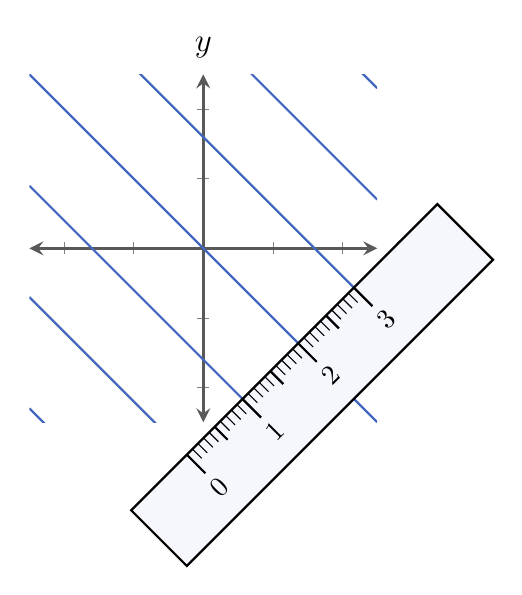
\begin{tikzpicture}
            \begin{axis}[
                xynogrid,
                width=6cm, height=6cm,
            ]
            \foreach \m in {-5,...,5}
                \addplot[hyperplane1D={xblue}] {-x+3.2*\m};
            \end{axis}
            \path[xshift=2cm, yshift=-1.825cm, opacity=1] pic[rotate=45, transform shape] (A) {ruler={5.5}{1}{1}{xblue!5}{}};
        \end{tikzpicture}
    \end{center}
    \caption{The graphical representation of a ruler shown next to the ruler, such that the infinite set of lines drawn match the ruler's graduation marks.}
    \label{fig:rulers_as_lines}
\end{marginfigure}

In $\Rs[3]$ a ruler is represented in a similar way, but with \textit{planes} instead of lines (\cref{fig:rulers_as_planes}). And in general, the rulers for a space $\Rs[n]$ can be represented using an infinite set of $(n-1)$-dimensional \textit{hyperplanes}.

\begin{marginfigure}
    \begin{center}
        \tdplotsetmaincoords{50}{110}
        \begin{tikzpicture}[tdplot_main_coords, rotate=0, scale=0.85]
            \pgfmathsetmacro{\a}{1.5}
            \pgfmathsetmacro{\b}{\a+0.5}
            \foreach \z in {-2,-1.25,...,2}
                \draw[very thick, xgreen, fill=xgreen, opacity=0.5] (-\a,-\a,\z) -- (-\a,\a,\z) -- (\a,\a,\z) -- (\a,-\a,\z) -- cycle;
        \end{tikzpicture}
        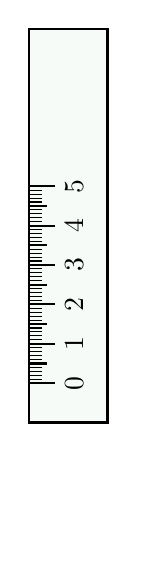
\begin{tikzpicture}
            \node (O) at (0,0) {};
            \path[above of=O, yshift=4.6mm] pic[rotate=90, transform shape] (A) {ruler={5}{1}{0.5}{xgreen!5}{}};
        \end{tikzpicture}
    \end{center}
    \caption{Representation of rulers in $\Rs[3]$ as planes.}
    \label{fig:rulers_as_planes}
\end{marginfigure}

From \cref{eq:ruler_measurement_explicit} we can see that any ruler $\dualvec{\alpha}$ can be written as the left half of an inner product, i.e. $\inner{\dualvec{\alpha}}{\cdot}$. This hints that the ruler is \textit{acting} on vectors, yielding a scalar. Looking at the explicit form of a ruler acting on a vector, we can see that not only do rulers represent linear functions, but they in-fact represent \textit{all} the possible \textit{linear} functions of the type $\phi:\Rs[n]\to\Rs$. Such functions are called \textit{linear forms}, or more specifically in this case a \textit{1-form}.

Since rulers can be represented as vectors but aren't exactly the same as \enquote{regular} vectors, they are also called \textit{dual vectors}, which is the name I will use for them from now on. For any vector space $\Rs[n]$, the dual vectors form a vector space of their own, called the \textit{dual space to $\Rs[n]$}.

The linearity of the dual vectors space simplifies many calculations - foremost, it allows us to construct dual vectors from other dual vectors using linear combinations. See \cref{example:dual_linear_comb} below.

\begin{example}{Linear combination of dual vectors}{dual_linear_comb}
   Suppose we have two dual vectors
    \begin{align}
        \dualvec{\alpha} &= \rowvec{1;-4;0},\\\nonumber
        \dualvec{\beta} &= \rowvec{2;1;3}.
        \label{eq:two_dual_vecs_in_R3}
    \end{align}

    We can use $\dualvec{\alpha}$ and $\dualvec{\beta}$ to create a third dual vector $\dualvec{\gamma}$:
    \begin{align}
        \dualvec{\gamma}&=5\rowvec{1;-4;0} + 2\rowvec{2;1;3}\\\nonumber  
                   &= \rowvec{5+4;-20+2;0+6}\\\nonumber
                   &= \rowvec{9;-18;6}.
        \label{eq:linear_comb_dual_vecs}
    \end{align}

    The application of $\dualvec{\gamma}$ on any vector $\vec{v}\in\Rs[3]$ is then given by
    \begin{equation}
        \inner{\dualvec{\gamma}}{\vec{v}} = 9v_{1} -18v_{2} +6v_{3},
        \label{eq:application_gamma_on_vec}
    \end{equation}
    which is exactly the application of $\dualvec{\alpha}$ on the vector five times followed by the application of $\dualvec{\beta}$ twice (try it for yourself!).
\end{example}

\subsection{Introducing some formalism}
Now that we know \textit{why} we use dual vectors, we can formalize the concept and find useful properties.

\begin{definition}{Dual space}{dual_space}
    Given a vector space $V$ over a field $\mathbb{F}$, its \textit{dual space}, denoted $\dualspace{V}$, is the set of all the linear functions $\phi:V\to\mathbb{F}$. The elements of $\dualspace{V}$ are called \textit{dual vectors}.
\end{definition}

A dual space equipped with a closed addition operation between any two of its elements and a closed product between its elements and the elements of the field $\mathbb{F}$ is itself a \textit{vector space}, with similar structure to the space $V$.

\begin{challenge}{Dual space as a vector space}{dual_vector_space_challange}
    Show that a dual space euipped with addition and scalar product as defined above is indeed a vector space (Use the definition XXX).
\end{challenge}

To write:
\begin{enumerate}
    \item Examples of dual vectors of functions?..
\end{enumerate}

\subsection{Basis sets and coordinate transformations}
\begin{enumerate}
    \item Dual basis: converting from a basis set in $V$ to its dual in $\dualspace{V}$.
    \item Covariance of dual vectors basis change vs. contra-varience of vectors.
\end{enumerate}
% ---------------------------------------------------------------- %
% STUFF I MIGHT NEED LATER...
%
% \begin{marginfigure}
%     \begin{center}
%         \begin{tikzpicture}
%             \begin{axis}[
%                 xyplane,
%                 width=7cm, height=7cm,
%             ]
%             % \draw[vector={xblue}] (0,0) -- (2,-3);
%             \addplot[name path=A, function={xred}] {6*exp(-x^2/2)-2};
%             \addplot[name path=B, function={xblue}] {5/(1+exp(-x))};
%             \addplot[xpurple, fill opacity=0.2] fill between[of=A and B, soft clip={domain=.5:5}];
%             \addplot[xgreen, fill opacity=0.2] fill between[of=A and B, soft clip={domain=-1:0.5}];
%             \end{axis}
%         \end{tikzpicture}
%     \end{center}
%     \caption{Drawing functions.}
%     \label{fig:funcs_test}
% \end{marginfigure}

% \begin{marginfigure}
%     \begin{center}
%         \begin{tikzpicture}
%             \begin{axis}[
%                 xyplane,
%                 width=7cm, height=7cm,
%             ]
%                 \pgfmathsetmacro{\ax}{3}
%                 \pgfmathsetmacro{\ay}{0.5}
%                 \pgfmathsetmacro{\bx}{-2}
%                 \pgfmathsetmacro{\by}{4}
%                 \pgfmathsetmacro{\tha}{atan2(\ay,\ax)}
%                 \pgfmathsetmacro{\thb}{atan2(\by,\bx)}
%                 \pgfmathsetmacro{\angL}{1.75}
%                 \coordinate (a) at (axis direction cs:\ax,\ay);
%                 \coordinate (b) at (axis direction cs:\bx,\by);
%
%                 % Draw
%                 \draw[ultra thick, dashed, xgreen, fill=xgreen, fill opacity=0.25, arcnode={6}{$\theta$}, text opacity=1] (0,0) -- ({\angL*cos(\tha)},{\angL*sin(\tha)}) arc (\tha:\thb:\angL) -- cycle;
%                 \draw[vector={xred}] (0,0) -- ++(a) node[pos=1.1] {$\vec{a}$};
%                 \draw[vector={xblue}] (0,0) -- ++(b) node[pos=1.1] {$\vec{b}$};
%             \end{axis}
%         \end{tikzpicture}
%     \end{center}
%     \caption{Drawing vectors.}
%     \label{fig:vecs_test}
% \end{marginfigure}

% \begin{figure}
%     \begin{center}
%         \tdplotsetmaincoords{50}{110}
%         \begin{tikzpicture}[tdplot_main_coords, rotate=0, scale=0.85]
%             \pgfmathsetmacro{\a}{1.5}
%             \pgfmathsetmacro{\b}{\a+0.5}
%             \foreach \z in {-2,-1.25,...,2}
%                 \draw[very thick, xblue, fill=xblue, opacity=0.5] (-\a,-\a,\z) -- (-\a,\a,\z) -- (\a,\a,\z) -- (\a,-\a,\z) -- cycle;
%             \draw[vector={xdarkblue}] (-\b,\b,-1.5) -- (-\b,\b,1.5);
%         \end{tikzpicture}
%         \hfill
%         \tdplotsetmaincoords{40}{120}
%         \begin{tikzpicture}[tdplot_main_coords, rotate=105, scale=0.85]
%             \pgfmathsetmacro{\a}{1.5}
%             \pgfmathsetmacro{\b}{\a+0.5}
%             \foreach \z in {-3,-1.5,...,3}
%                 \draw[very thick, xdarkgreen, fill=xgreen, opacity=0.5] (-\a,-\a,\z) -- (-\a,\a,\z) -- (\a,\a,\z) -- (\a,-\a,\z) -- cycle;
%             \draw[vector={xdarkgreen}] (-\b,\b,-1) -- (-\b,\b,1);
%         \end{tikzpicture}
%     \end{center}
%     \caption{Representation of rulers in $\Rs[3]$; as with the lines in the case of $\Rs[2]$, I added a vector showing the direction and density of the graduation marks. Note how the planes (stacks) in blue are more densely spaced compared to the green planes, and therefore the vector representing that respective ruler is longer compared to the vector representing the ruler in green.}
%     \label{fig:rulers_3D}
% \end{figure}

% \section{The Braket Notation and Einstein's Summation}

% \section{Quaternions and Octanions}

\section{Further Reading}


% - Geometric algebra
\chapter{Geometric Algebra}
\def\input@path{{./parts/background/geometric_algebra}}
\section{Preface}
\newthought{The goal of this chapter} is not to teach you, the reader, linear algebra from scratch - nor to be a thorough source of information on the topic. Rather, my aim is to overview the topic in such a way that new-comers, as well as those who studied linear algebra in an undergraduate university course, will gain the important insights of the topic needed for understanding the rest of the background material and spinors as well.

Instead of teaching the topic from the ground-up, like mathematicians tend to do\sidenote{In my view, courses that \enquote{build} linear algebra step-by-step give the students good knowledge of the structures of vector spaces, but tend to miss the intuitive view of what these structures can \textit{do}. This is exactly the difference between the \enquote{pure} mathematics of the mathematician and the mathematics as a tool of the scientist.}, I prefer to stick to the geometric interpretation of the vector spaces $\Rs[2]$ and $\Rs[3]$ (and to a lesser extent $\Rs[n]$ in general). These interpretations can be visualized relatively easily, and thus help in setting up the needed intuition in the student's mind, which becomes handy when the topic turns to more abstract constructs (such as for example vector spaces of matrices or functions).

In my personal experiences, when I was studying the topic I completely failed to understand it (and indeed, failed the courses I took) until it \enquote{clicked} for me in regards to 2- and 3-dimensional real spaces, i.e. - visible geometry. Then I didn't even have to study for exams anymore, as everything became clear enough to grasp and develop on the spot even during an exam (except for later, more advances concepts). That is why, for example, I absolutely adore courses and study materials of the topic\sidenote{And other mathematical topics as well.} which use animation, such as \textit{3Blue1Brown} great video essay series \href{https://www.3blue1brown.com/topics/linear-algebra}{Essence of linear algebra}\sidenote{Temporary sidenote which should become a citation for the mentioned 3B1B video series}.

There are very few proofs in this chapter, and those that are shown are not completely rigorous. For more in-depth materials, see the last section (further read). With that out of the way - let's begin!
\newpage


% - Abstract algebra
\chapter{Abstract Algebra}
\def\input@path{{./parts/background/abstract_algebra}}
\section{Preface}
\newthought{The goal of this chapter} is not to teach you, the reader, linear algebra from scratch - nor to be a thorough source of information on the topic. Rather, my aim is to overview the topic in such a way that new-comers, as well as those who studied linear algebra in an undergraduate university course, will gain the important insights of the topic needed for understanding the rest of the background material and spinors as well.

Instead of teaching the topic from the ground-up, like mathematicians tend to do\sidenote{In my view, courses that \enquote{build} linear algebra step-by-step give the students good knowledge of the structures of vector spaces, but tend to miss the intuitive view of what these structures can \textit{do}. This is exactly the difference between the \enquote{pure} mathematics of the mathematician and the mathematics as a tool of the scientist.}, I prefer to stick to the geometric interpretation of the vector spaces $\Rs[2]$ and $\Rs[3]$ (and to a lesser extent $\Rs[n]$ in general). These interpretations can be visualized relatively easily, and thus help in setting up the needed intuition in the student's mind, which becomes handy when the topic turns to more abstract constructs (such as for example vector spaces of matrices or functions).

In my personal experiences, when I was studying the topic I completely failed to understand it (and indeed, failed the courses I took) until it \enquote{clicked} for me in regards to 2- and 3-dimensional real spaces, i.e. - visible geometry. Then I didn't even have to study for exams anymore, as everything became clear enough to grasp and develop on the spot even during an exam (except for later, more advances concepts). That is why, for example, I absolutely adore courses and study materials of the topic\sidenote{And other mathematical topics as well.} which use animation, such as \textit{3Blue1Brown} great video essay series \href{https://www.3blue1brown.com/topics/linear-algebra}{Essence of linear algebra}\sidenote{Temporary sidenote which should become a citation for the mentioned 3B1B video series}.

There are very few proofs in this chapter, and those that are shown are not completely rigorous. For more in-depth materials, see the last section (further read). With that out of the way - let's begin!
\newpage


% - Lie groups and algebras
\chapter{Lie Groups and Algebras}
\def\input@path{{./parts/background/lie_groups_algebras}}
\section{Preface}
\newthought{The goal of this chapter} is not to teach you, the reader, linear algebra from scratch - nor to be a thorough source of information on the topic. Rather, my aim is to overview the topic in such a way that new-comers, as well as those who studied linear algebra in an undergraduate university course, will gain the important insights of the topic needed for understanding the rest of the background material and spinors as well.

Instead of teaching the topic from the ground-up, like mathematicians tend to do\sidenote{In my view, courses that \enquote{build} linear algebra step-by-step give the students good knowledge of the structures of vector spaces, but tend to miss the intuitive view of what these structures can \textit{do}. This is exactly the difference between the \enquote{pure} mathematics of the mathematician and the mathematics as a tool of the scientist.}, I prefer to stick to the geometric interpretation of the vector spaces $\Rs[2]$ and $\Rs[3]$ (and to a lesser extent $\Rs[n]$ in general). These interpretations can be visualized relatively easily, and thus help in setting up the needed intuition in the student's mind, which becomes handy when the topic turns to more abstract constructs (such as for example vector spaces of matrices or functions).

In my personal experiences, when I was studying the topic I completely failed to understand it (and indeed, failed the courses I took) until it \enquote{clicked} for me in regards to 2- and 3-dimensional real spaces, i.e. - visible geometry. Then I didn't even have to study for exams anymore, as everything became clear enough to grasp and develop on the spot even during an exam (except for later, more advances concepts). That is why, for example, I absolutely adore courses and study materials of the topic\sidenote{And other mathematical topics as well.} which use animation, such as \textit{3Blue1Brown} great video essay series \href{https://www.3blue1brown.com/topics/linear-algebra}{Essence of linear algebra}\sidenote{Temporary sidenote which should become a citation for the mentioned 3B1B video series}.

There are very few proofs in this chapter, and those that are shown are not completely rigorous. For more in-depth materials, see the last section (further read). With that out of the way - let's begin!
\newpage


%% -- PART 2: Spinors -- %%
\part{Spinors}


\makeatother
\end{document}
